\documentclass[11pt,a4paper]{article}

\usepackage[utf8]{inputenc}
\usepackage{amsmath,amssymb}
\usepackage{booktabs,tabularx}
\usepackage{geometry}
\usepackage{hyperref}
\usepackage{xcolor}
\usepackage{listings}
\usepackage{fancyhdr}
\usepackage{tikz}
\usepackage{enumitem}
\usetikzlibrary{arrows.meta,positioning,shapes.geometric,fit}

\geometry{margin=2.2cm,top=2.5cm,bottom=2.5cm}

\hypersetup{
  colorlinks=true,
  linkcolor=blue!60!black,
  urlcolor=blue!60!black,
  pdftitle={ISLS E1 — PCR-Conformant HDAG Codegen},
  pdfauthor={Sebastian Klemm},
}

\definecolor{codegreen}{rgb}{0.25,0.49,0.25}
\definecolor{codegray}{rgb}{0.5,0.5,0.5}
\definecolor{codeblue}{rgb}{0.15,0.3,0.55}
\definecolor{codebg}{rgb}{0.96,0.96,0.96}

\lstset{
  basicstyle=\ttfamily\scriptsize,
  breaklines=true,
  frame=single,
  backgroundcolor=\color{codebg},
  keywordstyle=\color{codeblue}\bfseries,
  commentstyle=\color{codegreen}\itshape,
  stringstyle=\color{red!60!black},
  numbers=left,
  numberstyle=\tiny\color{codegray},
  numbersep=5pt,
  tabsize=4,
  showstringspaces=false,
  language=Rust,
  morekeywords={async,await,impl,pub,mod,use,fn,let,mut,struct,enum,match,
    for,if,else,return,self,Self,crate,super,move,where,dyn,Box,Vec,
    String,Option,Result,Ok,Err,Some,None,trait,type},
}

\pagestyle{fancy}
\fancyhf{}
\fancyhead[L]{\small ISLS E1 --- PCR HDAG Codegen}
\fancyhead[R]{\small Klemm, 2026}
\fancyfoot[C]{\thepage}

\newcommand{\must}{\textbf{MUST}}
\newcommand{\mustnot}{\textbf{MUST NOT}}
\newcommand{\should}{\textbf{SHOULD}}

\begin{document}

\begin{titlepage}
\begin{center}
\vspace*{1cm}
{\Huge\bfseries ISLS v3.4}\\[0.3cm]
{\Huge\bfseries PCR-Conformant}\\[0.2cm]
{\Huge\bfseries HDAG Codegen Pipeline}\\[1cm]
{\LARGE Durchschlag 1: Die Zündung}\\[1.5cm]
{\Large Sebastian Klemm}\\[0.3cm]
{\small März 2026}\\[2cm]

{\itshape
Fehler werden nicht nachher gefixt.\\
Sie entstehen nicht.\\[0.3cm]
Der Hypercube-HDAG ist nicht nur für Entities.\\
Er ist der Codegen-Graph selbst.\\
Jede Datei ist ein Knoten. Jede Abhängigkeit eine Kante.\\
Topologische Traversierung garantiert vollständigen Kontext.\\[0.3cm]
Strukturelle Dateien sind deterministische Materialisierungen.\\
Null LLM-Tokens. Null Fehler. Per Konstruktion.
}

\vfill
\begin{tabular}{ll}
\textbf{Formaler Rahmen:} & PSP Master Spec v1.0 (Klemm, 2026) \\
\textbf{Datenstruktur:} & Hypercube-HDAG Framework (Klemm, 2025) \\
\textbf{Laufzeit:} & Program Cube Runtime v1.0 (Klemm, 2026) \\
\textbf{Crate:} & \texttt{isls-forge-llm} \\
\textbf{Neue Module:} & \texttt{hdag.rs}, \texttt{structural.rs}, \texttt{staged\_closure.rs}, \texttt{provided.rs} \\
\end{tabular}
\end{center}
\end{titlepage}

\tableofcontents
\newpage

% ============================================================
\section{Prinzip}

\subsection{Das Problem}

Die aktuelle Codegen-Pipeline generiert Dateien sequentiell und hofft,
dass Import-Pfade, Modul-Sichtbarkeit und Funktionsnamen stimmen.
Das LLM rät Pfade. Der Compiler findet Fehler. Ein Fix-Loop
repariert sie. Das ist Symptombehandlung.

In drei Runden Prompt-Optimierung: 80 $\to$ 55 $\to$ 100 Fehler.
Es wird schlimmer, nicht besser.

\subsection{Die Lösung}

Der Hypercube-HDAG wird vom Entity-Dekomposer zum \textbf{Codegen-Graphen}
erweitert. Jede Quelldatei ist ein HDAG-Knoten. Jede Abhängigkeit ist
eine typisierte Kante. Topologische Traversierung erzwingt, dass jeder
Knoten zum Generierungszeitpunkt den \textbf{vollständigen Kontext}
aller Vorgänger hat.

Das LLM rät keine Import-Pfade. Der HDAG sagt sie ihm.
Strukturelle Dateien werden nicht vom LLM generiert.
Sie sind deterministische Funktionen der Entity-Liste.

\subsection{Formale Verankerung}

\begin{center}
\begin{tabular}{lll}
\toprule
\textbf{PSP-Konzept} & \textbf{ISLS-Instanz} & \textbf{Referenz} \\
\midrule
Zustandsraum $\Sigma$ & TypeContext & PSP §II.1 \\
Operator $\Omega: \Sigma \to \Sigma$ & LLM-Generierung pro Knoten & PSP §III.1 \\
Programm $P = \Omega_k \circ \cdots \circ \Omega_1$ & HDAG-Traversierung & PSP §III.2 \\
Run Descriptor RD & AppSpec + Oracle-Config & PCR §5.3 \\
Determinism Contract & Identische Eingabe $\Rightarrow$ identischer Output & PSP §I.4 \\
Staged Closure & S0--S7 Pipeline & PCR §6.1 \\
Gate-Operator & \texttt{cargo check} & PSP §III.7 \\
Emission & Funktionierendes Projekt & Metatron §5.2 \\
\bottomrule
\end{tabular}
\end{center}

% ============================================================
\section{Der Codegen-HDAG}

\subsection{Definition}

\begin{quote}
\textbf{Definition (Codegen-HDAG).} Ein Codegen-HDAG ist ein Tupel
$G = (V, E, \tau, \Pi)$ wobei:
\begin{itemize}[nosep]
\item $V = \{v_1, \ldots, v_m\}$ ist die Menge der Datei-Knoten
\item $E \subseteq V \times V$ ist die Menge der Abhängigkeitskanten (azyklisch)
\item $\tau: V \to \{\textsc{Structural}, \textsc{Llm}\}$ klassifiziert jeden Knoten
\item $\Pi: E \to \mathcal{P}(\textsc{ProvidedSymbol})$ ordnet jeder Kante die
      bereitgestellten Symbole zu
\end{itemize}
\end{quote}

\subsection{Knoten-Klassifikation}

\textbf{Strukturelle Knoten} ($\tau(v) = \textsc{Structural}$) haben
vorbestimmten Inhalt. Sie werden aus der Entity-Liste konstruiert,
nicht vom LLM generiert. Kein Token-Verbrauch. Kein Fehlerpotential.

\textbf{LLM-Knoten} ($\tau(v) = \textsc{Llm}$) werden vom LLM generiert.
Ihr Prompt enthält \textbf{exakt} die Symbole die ihre eingehenden
Kanten bereitstellen --- nicht mehr, nicht weniger.

\subsection{Kanten und bereitgestellte Symbole}

Jede Kante $(v_i, v_j) \in E$ trägt eine Menge von Symbolen
$\Pi(v_i, v_j)$. Ein Symbol ist ein Tupel:

\begin{lstlisting}
pub struct ProvidedSymbol {
    pub import_path: String,    // "crate::errors::AppError"
    pub kind: SymbolKind,       // Enum, Struct, Trait, Function
    pub signature: String,      // volle Typdefinition
}
\end{lstlisting}

Wenn $v_j$ generiert wird, erhält das LLM die Vereinigung aller
Symbole seiner Vorgängerkanten:

\begin{equation}
\text{Context}(v_j) = \bigcup_{(v_i, v_j) \in E} \Pi(v_i, v_j)
\end{equation}

Das LLM \must{} genau diese Imports verwenden. Keine anderen.

% ============================================================
\section{Schichtarchitektur}

\subsection{Layer 0: Deterministische Materialisierung}

Diese Dateien sind \textbf{nicht LLM-generiert}. Sie sind
deterministische Funktionen der Entity-Liste.

\begin{center}
\scriptsize
\begin{tabular}{llp{6cm}}
\toprule
\textbf{Datei} & \textbf{Generator} & \textbf{Logik} \\
\midrule
\texttt{main.rs} & \texttt{generate\_main\_rs()} & mod-Deklarationen, Pool, Migrations, CORS, Routes \\
\texttt{models/mod.rs} & \texttt{generate\_models\_mod()} & \texttt{pub mod} + \texttt{pub use} pro Entity \\
\texttt{database/mod.rs} & \texttt{generate\_database\_mod()} & \texttt{pub mod pool;} + \texttt{pub mod X\_queries;} pro Entity \\
\texttt{services/mod.rs} & \texttt{generate\_services\_mod()} & \texttt{pub mod} pro Entity \\
\texttt{api/mod.rs} & \texttt{generate\_api\_mod()} & \texttt{pub mod}, \texttt{configure\_routes()}, Health Check \\
\texttt{migrations/*.sql} & \texttt{generate\_migration()} & FK-topologisch sortierte CREATE TABLEs, Seed-User \\
\texttt{Cargo.toml} & \texttt{generate\_cargo\_toml()} & Alle Dependencies, \texttt{[workspace]} Marker \\
\texttt{Dockerfile} & \texttt{generate\_dockerfile()} & rust:1.85-slim, Multi-Stage Build \\
\texttt{docker-compose.yml} & \texttt{generate\_docker\_compose()} & PostgreSQL + Backend + Frontend \\
\texttt{nginx.conf} & \texttt{generate\_nginx\_conf()} & Proxy \texttt{/api/} $\to$ backend:8080 \\
\texttt{.env.example} & \texttt{generate\_env()} & DATABASE\_URL, JWT\_SECRET, PORT \\
\texttt{frontend/*} & \texttt{generate\_frontend()} & Login, Entity-Seiten, API-Client \\
\bottomrule
\end{tabular}
\end{center}

\subsubsection{main.rs}

\begin{lstlisting}
fn generate_main_rs(spec: &AppSpec) -> String {
    format!(r#"mod api;
mod auth;
mod config;
mod database;
mod errors;
mod models;
mod pagination;
mod services;

use actix_web::{{web, App, HttpServer, middleware::Logger}};
use actix_cors::Cors;
use tracing_subscriber::EnvFilter;

#[actix_web::main]
async fn main() -> std::io::Result<()> {{
    dotenvy::dotenv().ok();
    tracing_subscriber::fmt()
        .with_env_filter(EnvFilter::from_default_env())
        .init();
    let pool = database::create_pool().await
        .expect("Failed to connect to database");
    let migration_sql = include_str!("../migrations/001_initial.sql");
    sqlx::raw_sql(migration_sql).execute(&pool).await
        .expect("Failed to run migrations");
    tracing::info!("Starting {name} on 0.0.0.0:8080");
    HttpServer::new(move || {{
        App::new()
            .app_data(web::Data::new(pool.clone()))
            .wrap(Cors::permissive())
            .wrap(Logger::default())
            .configure(api::configure_routes)
    }})
    .bind("0.0.0.0:8080")?
    .run()
    .await
}}"#, name = spec.name)
}
\end{lstlisting}

\subsubsection{models/mod.rs}

\begin{lstlisting}
fn generate_models_mod(spec: &AppSpec) -> String {
    let mut s = String::new();
    for entity in &spec.entities {
        s.push_str(&format!("pub mod {};\n", entity.snake_name()));
    }
    s.push('\n');
    for entity in &spec.entities {
        let sn = entity.snake_name();
        let pn = &entity.name;
        s.push_str(&format!(
            "pub use {}::{{{}, Create{}Payload, Update{}Payload}};\n",
            sn, pn, pn, pn
        ));
    }
    s
}
\end{lstlisting}

\subsubsection{database/mod.rs}

\begin{lstlisting}
fn generate_database_mod(spec: &AppSpec) -> String {
    let mut s = String::from("pub mod pool;\n");
    for entity in &spec.entities {
        s.push_str(&format!("pub mod {}_queries;\n", entity.snake_name()));
    }
    s.push_str("\npub use pool::create_pool;\n");
    s
}
\end{lstlisting}

\subsubsection{api/mod.rs}

\begin{lstlisting}
fn generate_api_mod(spec: &AppSpec) -> String {
    let mut s = String::from("pub mod auth_routes;\n");
    for entity in &spec.entities {
        s.push_str(&format!("pub mod {};\n", entity.snake_name()));
    }
    s.push_str("\nuse actix_web::{web, HttpResponse, Responder};\n\n");
    s.push_str("pub fn configure_routes(cfg: &mut web::ServiceConfig) {\n");
    s.push_str("    auth_routes::auth_routes(cfg);\n");
    for entity in &spec.entities {
        let sn = entity.snake_name();
        s.push_str(&format!("    {}::{}_routes(cfg);\n", sn, sn));
    }
    s.push_str("    cfg.route(\"/api/health\", web::get().to(health_check));\n");
    s.push_str("}\n\n");
    s.push_str(concat!(
        "async fn health_check(pool: web::Data<sqlx::PgPool>)",
        " -> impl Responder {\n",
        "    match sqlx::query(\"SELECT 1\")",
        ".execute(pool.get_ref()).await {\n",
        "        Ok(_) => HttpResponse::Ok().json(",
        "serde_json::json!({",
        "\"status\":\"ok\",\"database\":\"connected\"",
        ",\"version\":\"1.0.0\"})),\n",
        "        Err(_) => HttpResponse::ServiceUnavailable().json(",
        "serde_json::json!({\"status\":\"error\"",
        ",\"database\":\"disconnected\"})),\n",
        "    }\n}\n"));
    s
}
\end{lstlisting}

\subsubsection{migrations/001\_initial.sql}

\begin{lstlisting}
fn generate_migration(spec: &AppSpec) -> String {
    let sorted = topological_sort_entities(&spec.entities);
    let mut sql = String::new();
    for entity in &sorted {
        sql.push_str(&format!(
            "CREATE TABLE IF NOT EXISTS {} (\n    id BIGSERIAL PRIMARY KEY,\n",
            entity.table_name()));
        for field in &entity.fields {
            let pg = rust_type_to_pg(&field.field_type, field.nullable);
            let nn = if field.nullable { "" } else { " NOT NULL" };
            sql.push_str(&format!("    {} {}{},\n", field.name, pg, nn));
        }
        for fk in &entity.foreign_keys {
            sql.push_str(&format!(
                "    {}_id BIGINT REFERENCES {}(id),\n",
                fk.target.to_snake_case(), fk.target_table()));
        }
        sql.push_str(
            "    created_at TIMESTAMPTZ NOT NULL DEFAULT NOW(),\n\
             \x20   updated_at TIMESTAMPTZ NOT NULL DEFAULT NOW()\n);\n\n");
    }
    // Seed admin with bcrypt hash computed at generation time
    let hash = bcrypt::hash("admin123", 12).expect("bcrypt");
    sql.push_str(&format!(
        "INSERT INTO users (email, password_hash, role, is_active) \
         VALUES ('admin@example.com', '{}', 'admin', true) \
         ON CONFLICT (email) DO NOTHING;\n", hash));
    sql
}
\end{lstlisting}

\subsection{Layer 1--7: LLM-generierte Dateien}

\begin{center}
\scriptsize
\begin{tabular}{clll}
\toprule
\textbf{Layer} & \textbf{Dateien} & \textbf{Abhängigkeiten} & \textbf{Rolle} \\
\midrule
1 & \texttt{errors.rs}, \texttt{pagination.rs}, \texttt{config.rs} & keine & Fundament \\
2 & \texttt{auth.rs} & L1 (errors) & Auth-Infrastruktur \\
3 & \texttt{models/\{entity\}.rs} $\times N$ & L1 (errors) & Entity-Structs + Payloads \\
4 & \texttt{database/pool.rs} & L1 (errors) & PgPool-Erstellung \\
5 & \texttt{database/\{entity\}\_queries.rs} $\times N$ & L1, L3, L4 & SQL-Queries \\
6 & \texttt{services/\{entity\}.rs} $\times N$ & L1, L3, L5 & Business-Logik \\
7 & \texttt{api/\{entity\}.rs} $\times N$, \texttt{api/auth\_routes.rs} & L1, L2, L3, L6 & HTTP-Routes \\
\bottomrule
\end{tabular}
\end{center}

Innerhalb jedes Layers können Knoten parallel generiert werden
(keine Abhängigkeiten untereinander). Die topologische Sortierung
erzwingt die Layer-Reihenfolge automatisch.

% ============================================================
\section{Typisierte Kanten: ProvidedSymbol}

\subsection{Kantendefinition}

Jede Kante $(v_i, v_j)$ trägt die Menge der Symbole die $v_i$
für $v_j$ bereitstellt:

\begin{lstlisting}
pub struct HdagEdge {
    pub from: usize,         // Quell-Knoten
    pub to: usize,           // Ziel-Knoten
    pub provides: Vec<ProvidedSymbol>,
}

pub struct ProvidedSymbol {
    pub import_path: String, // "crate::errors::AppError"
    pub kind: SymbolKind,    // Enum, Struct, Trait, Function
    pub signature: String,   // volle Typdefinition fuer Prompt
}

pub enum SymbolKind { Enum, Struct, Trait, Function, Module }
\end{lstlisting}

\subsection{Konkrete Kanten-Templates}

\subsubsection{errors $\to$ *}

\begin{lstlisting}
fn provides_apperror() -> Vec<ProvidedSymbol> {
    vec![ProvidedSymbol {
        import_path: "crate::errors::AppError".into(),
        kind: SymbolKind::Enum,
        signature: r#"#[derive(Debug, Serialize)]
pub enum AppError {
    NotFound(String),
    InternalError(String),
    ValidationError(Vec<String>),
    Unauthorized,
    Forbidden,
}
impl actix_web::ResponseError for AppError { ... }"#.into(),
    }]
}
\end{lstlisting}

\subsubsection{pagination $\to$ *}

\begin{lstlisting}
fn provides_pagination() -> Vec<ProvidedSymbol> {
    vec![
        ProvidedSymbol {
            import_path: "crate::pagination::PaginationParams".into(),
            kind: SymbolKind::Struct,
            signature: "#[derive(Debug, Deserialize)]\n\
                pub struct PaginationParams {\n\
                \x20   pub page: Option<i64>,\n\
                \x20   pub per_page: Option<i64>,\n}".into(),
        },
        ProvidedSymbol {
            import_path: "crate::pagination::PaginatedResponse".into(),
            kind: SymbolKind::Struct,
            signature: "#[derive(Debug, Serialize)]\n\
                pub struct PaginatedResponse<T: Serialize> {\n\
                \x20   pub items: Vec<T>,\n\
                \x20   pub total: i64, pub page: i64,\n\
                \x20   pub per_page: i64,\n}".into(),
        },
    ]
}
\end{lstlisting}

\subsubsection{auth $\to$ *}

\begin{lstlisting}
fn provides_authuser() -> Vec<ProvidedSymbol> {
    vec![ProvidedSymbol {
        import_path: "crate::auth::AuthUser".into(),
        kind: SymbolKind::Struct,
        signature: "pub struct AuthUser {\n\
            \x20   pub user_id: i64,\n\
            \x20   pub email: String,\n\
            \x20   pub role: String,\n}".into(),
    }]
}
\end{lstlisting}

\subsubsection{model $\to$ queries/services/routes (dynamisch pro Entity)}

\begin{lstlisting}
fn provides_model_types(entity: &EntityDef) -> Vec<ProvidedSymbol> {
    let sn = entity.snake_name();
    let pn = &entity.name;
    // Build struct signature from entity fields
    let mut sig = format!(
        "#[derive(Debug, Serialize, Deserialize, FromRow)]\n\
         pub struct {} {{\n    pub id: i64,\n", pn);
    for field in &entity.fields {
        sig.push_str(&format!("    pub {}: {},\n",
            field.name, field_to_rust_type(field)));
    }
    sig.push_str("    pub created_at: DateTime<Utc>,\n\
                  \x20   pub updated_at: DateTime<Utc>,\n}");
    vec![
        ProvidedSymbol {
            import_path: format!("crate::models::{}::{}", sn, pn),
            kind: SymbolKind::Struct,
            signature: sig,
        },
        ProvidedSymbol {
            import_path: format!(
                "crate::models::{}::Create{}Payload", sn, pn),
            kind: SymbolKind::Struct,
            signature: format!(
                "#[derive(Debug, Deserialize)]\n\
                 pub struct Create{}Payload {{ ... }}", pn),
        },
        ProvidedSymbol {
            import_path: format!(
                "crate::models::{}::Update{}Payload", sn, pn),
            kind: SymbolKind::Struct,
            signature: format!(
                "#[derive(Debug, Deserialize)]\n\
                 pub struct Update{}Payload {{ ... }}", pn),
        },
    ]
}
\end{lstlisting}

% ============================================================
\section{Der HDAG-Prompt}

Das LLM erhält pro Knoten einen Prompt der \textbf{exakt} die
verfügbaren Symbole enthält --- nicht geraten, sondern vom HDAG
propagiert:

\begin{lstlisting}
fn build_hdag_prompt(
    path: &str,
    role: &FileRole,
    provided: &[ProvidedSymbol],
    context: &TypeContext,
) -> String {
    let mut p = String::new();
    p.push_str(&format!("Generate `{}`.\n\n", path));
    p.push_str(&role_description(role));

    // EXACT imports -- HDAG-determined, not guessed
    p.push_str("\n## AVAILABLE IMPORTS (use ONLY these):\n\n");
    for sym in provided {
        p.push_str(&format!("use {};  // {}\n",
            sym.import_path, sym.kind));
    }

    // Always-available crate imports
    p.push_str("\n## CRATE IMPORTS (always available):\n");
    p.push_str("use actix_web::{web, HttpResponse, Responder};\n");
    p.push_str("use sqlx::PgPool;\n");
    p.push_str("use sqlx::Row;  // needed for .get()\n");
    p.push_str("use serde::{Serialize, Deserialize};\n");
    p.push_str("use sqlx::FromRow;\n");
    p.push_str("use chrono::{DateTime, Utc};\n");
    p.push_str("use tracing::{info, warn, error};\n");

    // Full type signatures for predecessor types
    p.push_str("\n## TYPE SIGNATURES:\n\n");
    for sym in provided {
        if !sym.signature.is_empty() {
            p.push_str(&format!("// {}:\n{}\n\n",
                sym.import_path, sym.signature));
        }
    }

    // Universal rules
    p.push_str("\n## RULES:\n");
    p.push_str("- Output ONLY the complete Rust file\n");
    p.push_str("- Use ONLY the imports listed above\n");
    p.push_str("- sqlx: query_as::<_, T>(), NEVER query_as!()\n");
    p.push_str("- Pagination: i64 for page/per_page\n");
    p.push_str("- Nullable: Option<T>, clone before .bind()\n");
    p.push_str("- Routes return Result<impl Responder, AppError>\n");
    p.push_str("- Route config: pub fn {entity}_routes(\
                cfg: &mut web::ServiceConfig)\n");
    p
}
\end{lstlisting}

\subsection{Warum das Import-Fehler eliminiert}

\begin{enumerate}[nosep]
\item Das LLM sieht \texttt{use crate::errors::AppError} --- es
  schreibt diesen Import, nicht \texttt{use crate::AppError}.
\item Die Signatur von \texttt{AppError} enthält
  \texttt{\#[derive(Serialize)]} --- das LLM weiß, dass
  \texttt{.json(AppError::...)} funktioniert.
\item \texttt{PaginationParams} hat \texttt{i64}-Felder ---
  das LLM verwendet \texttt{i64}, nicht \texttt{u64}.
\item \texttt{sqlx::Row} ist in den Crate-Imports gelistet ---
  \texttt{.get(0)} funktioniert.
\item Die Regel ``clone Option fields before .bind()'' verhindert
  partial-move-Fehler.
\end{enumerate}

% ============================================================
\section{PCR Staged Closure}

Die Pipeline folgt der Staged Closure aus PCR §6.1:

\begin{center}
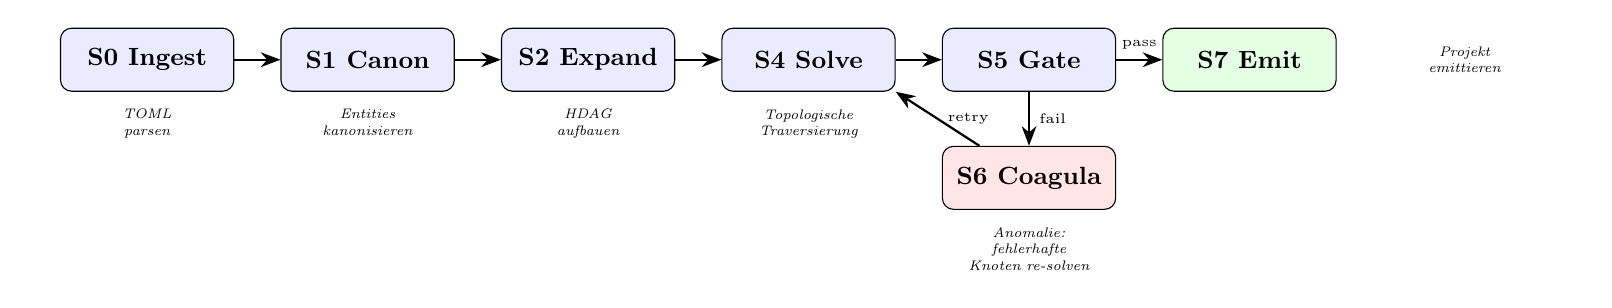
\begin{tikzpicture}[
  stage/.style={draw, rounded corners, fill=blue!8,
    minimum width=2.2cm, minimum height=0.8cm, font=\small\bfseries},
  arrow/.style={-{Stealth[length=2.5mm]}, thick},
  note/.style={font=\tiny\itshape, text width=2.8cm, align=center},
]

\node[stage] (s0) at (0,0) {S0 Ingest};
\node[stage] (s1) at (2.8,0) {S1 Canon};
\node[stage] (s2) at (5.6,0) {S2 Expand};
\node[stage] (s4) at (8.4,0) {S4 Solve};
\node[stage] (s5) at (11.2,0) {S5 Gate};
\node[stage, fill=red!10] (s6) at (11.2,-1.5) {S6 Coagula};
\node[stage, fill=green!10] (s7) at (14,0) {S7 Emit};

\draw[arrow] (s0) -- (s1);
\draw[arrow] (s1) -- (s2);
\draw[arrow] (s2) -- (s4);
\draw[arrow] (s4) -- (s5);
\draw[arrow] (s5) -- node[above,font=\tiny] {pass} (s7);
\draw[arrow] (s5) -- node[right,font=\tiny] {fail} (s6);
\draw[arrow] (s6) -- node[right,font=\tiny] {retry} (s4.south east);

\node[note, below=0.1cm] at (s0.south) {TOML\\parsen};
\node[note, below=0.1cm] at (s1.south) {Entities\\kanonisieren};
\node[note, below=0.1cm] at (s2.south) {HDAG\\aufbauen};
\node[note, below=0.1cm] at (s4.south) {Topologische\\Traversierung};
\node[note, right=0.1cm] at (s7.east) {Projekt\\emittieren};
\node[note, below=0.1cm] at (s6.south) {Anomalie:\\fehlerhafte\\Knoten re-solven};

\end{tikzpicture}
\end{center}

\subsection{S0 Ingest}

\texttt{warehouse.toml} $\to$ \texttt{AppSpec}. Entity-Liste,
Feld-Definitionen, FK-Beziehungen, Domain-Name.

\subsection{S1 Canon}

Entity-Namen kanonisieren (PascalCase), Feldnamen (snake\_case),
Tabellenamen (snake\_case, Plural). FK-Referenzen auflösen.

\subsection{S2 Expand}

Codegen-HDAG aufbauen. Knoten für jede Datei. Kanten für jede
Abhängigkeit. Typisierte Kanten mit \texttt{ProvidedSymbol}.
Layer-0-Knoten erhalten ihren Inhalt direkt.

\subsection{S4 Solve}

Topologische Sortierung des HDAG (Kahn's Algorithmus mit
deterministischem Tie-Break: lexikographisch nach Pfad).
Traversierung in sortierter Reihenfolge:
\begin{itemize}[nosep]
\item Strukturelle Knoten: Inhalt direkt auf Disk schreiben
\item LLM-Knoten: Prompt aus Vorgänger-Symbolen bauen,
  LLM aufrufen, Code schreiben, TypeContext aktualisieren
\end{itemize}

\subsection{S5 Gate}

\textbf{Ein} \texttt{cargo check} auf das vollständige Projekt.
\begin{itemize}[nosep]
\item 0 Fehler $\Rightarrow$ S7 Emit
\item $>0$ Fehler $\Rightarrow$ S6 Coagula (Anomalie)
\end{itemize}

\subsection{S6 Coagula (Anomalie-Pfad)}

\must{} als Anomalie geloggt werden. Nicht der Normalfall.

\begin{enumerate}[nosep]
\item Compiler-Fehler nach Datei gruppieren
\item Modul-Map von Disk lesen (die echten mod.rs-Dateien)
\item Pro fehlerhafte Datei: Fix-Prompt mit Fehlertext +
  Vorgänger-Symbole aus HDAG + Modul-Map
\item LLM regeneriert nur diese Datei
\item Zurück zu S5 Gate
\item Maximal 3 Zyklen. Dann \textbf{keine Emission}. Error-Report.
\end{enumerate}

\subsection{S7 Emit}

Deployment-Dateien (Dockerfile, docker-compose, nginx, Frontend)
sind bereits in Layer 0 geschrieben. Projekt ist vollständig.
Emission = das Projekt-Verzeichnis ist der Output.

% ============================================================
\section{Implementierung}

\subsection{Neue Dateien in \texttt{isls-forge-llm/src/}}

\begin{center}
\begin{tabular}{llp{7cm}}
\toprule
\textbf{Datei} & \textbf{ca. LOC} & \textbf{Inhalt} \\
\midrule
\texttt{hdag.rs} & 200 & \texttt{CodegenHdag}, \texttt{HdagNode}, \texttt{HdagEdge},
  \texttt{ProvidedSymbol}, \texttt{SymbolKind}, \texttt{topological\_sort()},
  \texttt{predecessors()}, \texttt{provided\_symbols()} \\
\texttt{structural.rs} & 350 & Alle \texttt{generate\_*}-Funktionen für Layer 0:
  main.rs, mod.rs-Dateien, Migration, Cargo.toml, Dockerfile, etc. \\
\texttt{provided.rs} & 200 & Alle \texttt{provides\_*}-Funktionen:
  \texttt{provides\_apperror()}, \texttt{provides\_pagination()},
  \texttt{provides\_authuser()}, \texttt{provides\_model\_types()}, etc. \\
\texttt{staged\_closure.rs} & 250 & \texttt{StagedClosure::execute()},
  S0--S7 Pipeline, Gate, Coagula \\
\bottomrule
\end{tabular}
\end{center}

\subsection{Änderungen an bestehenden Dateien}

\begin{itemize}[nosep]
\item \texttt{forge.rs}: \texttt{LlmForge::generate()} dispatcht zu
  \texttt{StagedClosure} für LLM-Modus, behält Mock-Pfad bei
\item \texttt{lib.rs}: Neue Module exportieren
\item \texttt{Cargo.toml}: \texttt{bcrypt} und \texttt{regex} als Dependencies
\end{itemize}

\subsection{Unverändert}

\begin{itemize}[nosep]
\item \texttt{mock.rs}: Mock-Generierung bleibt identisch
\item \texttt{prompt.rs}: Bestehende Prompts bleiben als Fallback,
  werden aber im HDAG-Pfad nicht verwendet (HDAG-Prompt ist eigenständig)
\item Alle anderen ISLS-Crates: keine Änderungen
\item Alle 527+ Tests: \must{} bestehen
\end{itemize}

% ============================================================
\section{Was eliminiert wird}

\begin{center}
\begin{tabular}{lll}
\toprule
\textbf{Fehlerklasse} & \textbf{Ursache bisher} & \textbf{Lösung} \\
\midrule
Falsche Import-Pfade & LLM rät & HDAG sagt exakte Pfade \\
Private Module (\texttt{mod} statt \texttt{pub mod}) & LLM generiert mod.rs & Layer 0: deterministisch \\
Fehlende mod-Deklarationen in main.rs & LLM vergisst & Layer 0: deterministisch \\
Falsche Funktionsnamen in api/mod.rs & LLM erfindet & Layer 0: deterministisch \\
\texttt{u64} statt \texttt{i64} & LLM kennt PaginationParams nicht & Signatur im Prompt \\
Fehlendes \texttt{use sqlx::Row} & LLM vergisst & Crate-Imports-Liste \\
Fehlendes \texttt{Serialize} auf AppError & LLM sieht Derive nicht & Signatur im Prompt \\
Partial moves bei Option-Feldern & LLM kennt Ownership nicht & Regel im Prompt \\
\bottomrule
\end{tabular}
\end{center}

% ============================================================
\section{Verifikation}

\subsection{ISLS-Workspace}

\begin{lstlisting}[language=bash]
cargo build --workspace --release
cargo test --workspace
# Alle 527+ Tests muessen bestehen
\end{lstlisting}

\subsection{LLM End-to-End}

\begin{lstlisting}[language=bash]
rm -rf output/warehouse
cargo run --release -p isls-cli -- forge-v2 \
    --requirements examples/warehouse.toml \
    --api-key $OPENAI_API_KEY \
    --output ./output/warehouse
# Erwartung: S0-S7 ohne S6 (kein Coagula noetig)

cd output/warehouse/backend && cargo build
# Erwartung: 0 Errors

cd .. && docker-compose up -d --build
# Erwartung: 3 Container starten

curl -sf http://localhost:8080/api/health
# Erwartung: {"status":"ok","database":"connected"}

TOKEN=$(curl -sf -X POST http://localhost:8080/api/auth/login \
  -H "Content-Type: application/json" \
  -d '{"email":"admin@example.com","password":"admin123"}' \
  | jq -r '.token')
# Erwartung: JWT Token

curl -sf -X POST http://localhost:8080/api/products \
  -H "Content-Type: application/json" \
  -H "Authorization: Bearer $TOKEN" \
  -d '{"sku":"WH-001","name":"Widget","unit_price_cents":1500}'
# Erwartung: Product JSON

docker-compose down -v
\end{lstlisting}

\subsection{Binäres Kriterium (Durchschlag 1)}

Ein Mensch öffnet einen Browser, loggt ein, legt ein Produkt an.
Ja oder Nein.

% ============================================================
\section{Constraints}

\begin{enumerate}[nosep]
\item Alle bestehenden 527+ ISLS-Tests \must{} bestehen.
\item Mock-Modus \must{} unverändert funktional bleiben.
\item Layer-0-Dateien werden \mustnot{} vom LLM generiert.
\item Der HDAG wird deterministisch aus der AppSpec gebaut.
\item Topologische Sortierung mit deterministischem Tie-Break (lexikographisch).
\item Jeder LLM-Prompt enthält \textbf{exakt} die bereitgestellten Symbole.
\item Das Gate (\texttt{cargo check}) läuft \textbf{einmal} nach vollständiger Generierung.
\item S6 Coagula ist der \textbf{Anomalie-Pfad}. Wird er ausgelöst, wird das geloggt.
\item Nach 3 Coagula-Zyklen: \textbf{keine Emission}. Error-Report stattdessen.
\item \texttt{bcrypt} \must{} in \texttt{isls-forge-llm/Cargo.toml} für Seed-Hash-Generierung sein.
\item Dockerfile \must{} \texttt{rust:1.85-slim} oder neuer verwenden.
\item Copyright: MIT. \textcopyright{} 2026 Sebastian Klemm.
\end{enumerate}

\vfill
\noindent\rule{\textwidth}{0.4pt}
\begin{center}
\small
ISLS v3.4 --- PCR-Conformant HDAG Codegen Pipeline\\
Sebastian Klemm --- März 2026\\
Durchschlag 1 der Nullpunkt-Kaskade.\\
Der Hypercube sequenziert. Die Trompete bläst.\\
\url{https://github.com/LashSesh/graphity}
\end{center}

\end{document}
